% What does the GUI want to achieve? High-level point?
% I don't understand what high-level points need to be made, it's clear what
% the GUI wants to achieve.

The user interface of the application focuses on the displayed
visualization, which takes up the majority of the window and can be maximised
to fill the available space. Other panels occupy the right and bottom sections
of the window.

The right panel is aimed at providing the user with options to adapt the shown data.
Choice of visualization is presented to the user by a list in the top of the
right panel, followed underneath by options specific to that visualisation, and
then by general filters to refine the processed data. If a recorded data source
is active, time controls are displayed on the right panel to allow the user to
adjust the speed at which data is processed and visualised by pausing,
doubling or halving the current data rate. 

The bottom panel shows fine and aggregate details of the
processed data. To fit the large amount of data available into such a limited
space, a tabbed pane is used on the left to categorise distinct types of data.
The right section of this panel contains a `Context Pane', which shows further detail of selected data on demand. The left
`Analysis' panel and the right `Context' panel are split in two by a split
pane, so the user can modify the proportion of each they wish to see.

% Compressed and merged the below paragraphs, I think it's important to explain
% about user messages, it's an important part of the interface.

Window tools, an exclusive-mode full screen option and the facility to select
a new data source are all accessed by the main menu bar. Messages to the user
come in the form of warning dialogues for user or program errors, notifications
in the bottom `Analysis' panel for program notifications, and text messages in
the bottom `Context' panel for help messages and suggestions. {\color{red} Include reference to figure}


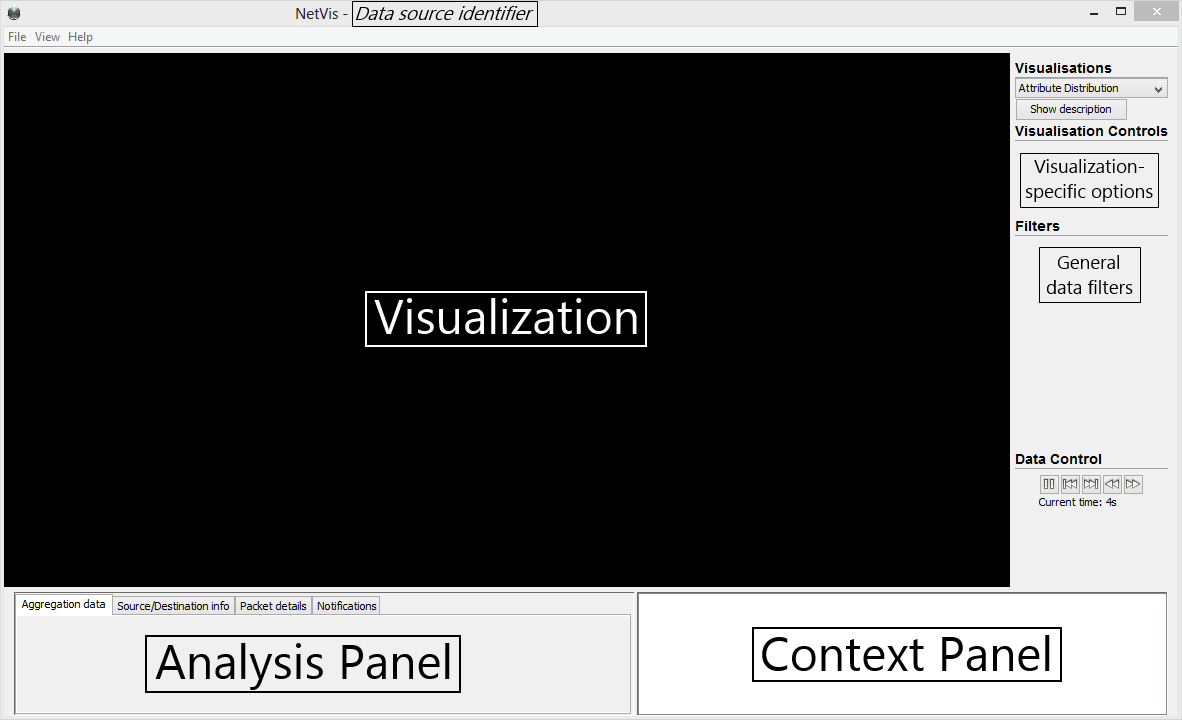
\includegraphics[width=\linewidth]{materials/layout-diagram.png}
